% 2D Example Points
%
% File:         2d-points.tex
% Author:       Bob Walton (walton@acm.org)
% Date:      	Wed Dec 19 08:19:59 EST 2012
  
\documentclass{minimal}
\usepackage[paperheight=2in,paperwidth=2in,
            height=2in,hoffset=0.05in,
	    voffset=0.05in,left=0in,width=2in]{geometry}
\usepackage{color}
\usepackage[usenames]{xcolor}
\usepackage{tikz}
\begin{document}
\raggedright
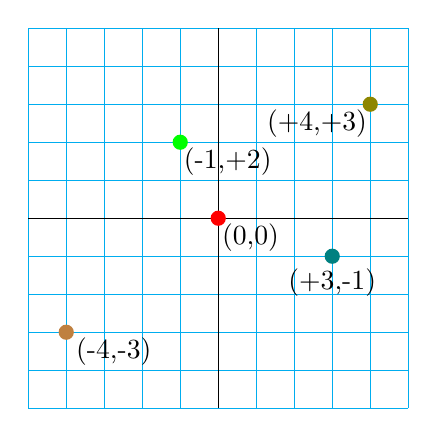
\begin{tikzpicture}[x=0.190in,y=0.190in]
\draw[cyan] (-5,-5) grid[step=1] (5,5);
\draw[black] (-5,0) -- (+5,0);
\draw[black] (0,-5) -- (0,+5);
\fill[red] (0,0) circle(0.2) + (+0.85,-0.5) node[black]{(0,0)};
\fill[green] (-1,+2) circle(0.2) + (+1.25,-0.5) node[black]{(-1,+2)};
\fill[teal] (+3,-1) circle(0.2) + (0,-0.7) node[black]{(+3,-1)};
\fill[brown] (-4,-3) circle(0.2) + (+1.25,-0.5) node[black]{(-4,-3)};
\fill[olive] (+4,+3) circle(0.2) + (-1.4,-0.5) node[black]{(+4,+3)};
\end{tikzpicture}
\end{document}
